\documentclass[11pt]{amsart}
\usepackage[margin=1in]{geometry}                % See geometry.pdf to learn the layout options. There are lots.
\geometry{letterpaper}                   % ... or a4paper or a5paper or ... 
%\geometry{landscape}                % Activate for for rotated page geometry
\usepackage[parfill]{parskip}    % Activate to begin paragraphs with an empty line rather than an indent
\usepackage{graphicx, enumerate}


\usepackage{subfig}
\usepackage[]{floatrow} 
\floatsetup[table]{style=plaintop}
\floatsetup[figure]{%style=BOXED, 
floatrowsep=qquad,   valign=c}
\floatsetup[subfigure]{subfloatrowsep=qquad, heightadjust=object, valign=c,  rowfill=yes}


\usepackage{amssymb}
\usepackage[normalem]{ulem}
\usepackage{epstopdf}
\DeclareGraphicsRule{.tif}{png}{.png}{`convert #1 `dirname #1`/`basename #1 .tif`.png}


\usepackage{tikz}
\usetikzlibrary{calc, through}
\usetikzlibrary{decorations.markings}
\usetikzlibrary{arrows}
\usetikzlibrary{positioning}

%\date{}                                           % Activate to display a given date or no date


\usepackage{hyperref}

%\newcommand{\deg}{\mathrm{deg}}

\newcommand{\bv}[1]{\ensuremath{\mathbf{#1}}}
\newcommand{\be}{\begin{enumerate}}
\newcommand{\ee}{\end{enumerate}}

\begin{document}
\begin{center}
\begin{Large} Math F307 \hfill Spring 2017

Homework Exercises 
\end{Large}
\end{center}
%\maketitle
%\section{}
%\subsection{}

\subsection*{Instructions for writing up homework}
\begin{itemize}
\item Although you are encouraged to work with your classmates on the homework assignments, you must write up the solutions individually.
\item Read the section!
 \item Use pen or non-smeary pencil. Do not have little scritchies on the side. 
 \item Staple your homework. 
 \item Write legibly, and leave lots of whitespace. Make sure your writing is dark enough to be readable. If this is problematic for you, consider typing your homework.
 \item Answer the question in complete sentences, where appropriate.
\item {\bf Write the \fbox{problem statements} as well as the answers. } This is not optional. \underline{Points will be deducted if you do not do this}.
\item Have headings indicating the section.
\item {\bf In the upper right hand corner of your top page,} write your name (first and last) on your assignment, along with the course number (Math 307) and which assignment it is.
\item {\bf You are expected to ask questions in class about the homework problems!}
\end{itemize}

\section*{Homework Set 8}

{\bf DUE Friday, March 31 \fbox{at the beginning of class}.}



\subsection*{Graph coloring and planar graphs}


%\subsection*{Additional Problems}

To turn in:
\be

\item Find the chromatic number  $\chi(G)$ of each of the graphs shown in Figure 1. To do so: (1) provide a coloring (with actual colors) for each of the graphs using $\chi(G)$ colors, and (2) explain why you cannot use fewer colors.

\item Give examples of a graph (that are not examples from class or the worksheet) for which 
\be
\item $\chi(G)  = \Delta(G)$
\item $\chi(G) < \Delta(G)$.
\ee

\item Suppose a graph $G$ has chromatic number 1. What can you say about $G$?

\item 
\be
\item Use the greedy algorithm to color the graph $G$ in Figure \ref{greedy}. How many colors did you use?
\item Determine the chromatic number of $G$. Justify that the number you find really is the number of colors needed.
\ee

\item
The math department is trying to schedule focus group interviews with students for certain classes outside of the ordinary class time. The courses have the following (entirely made up) student overlaps:

\begin{tabular}{c| c |c| c| c|c|c}
& Math 265 & Math 314 & Math 307 & Math 490 & Math  405 & Math 422 \\
\hline
Math 265 &  & 1 &  5 & 0 & 0&2\\ \hline
Math 314 & 1 &  & 0 & 0 & 0 & 0\\	\hline
Math 307 & 5 & 0 & & 1 & 0 & 2\\	\hline
Math 490 & 0 & 0 & 1&   &4& 2 \\ 	\hline
Math 405 & 0 & 0 & 0 & 4 & & 4 \\ \hline
Math 422 &2 & 0 & 2 & 2 &  4 & \\
\hline
\end{tabular}

\be
\item Construct a graph representing the student overlaps (that is, assign the vertices to be the classes, and connect the vertices with an edge if there are students in both classes, labelled with the number of students in both classes).

\item How many meeting times are needed? Explain, briefly. 

\item Suppose only three meeting times are available, at 9AM, 10AM and 11AM, and furthermore, suppose that only one class is allowed to meet at 9AM.  Is it possible to schedule the focus groups with this restriction? If so, give a possible schedule. If not, explain why not.

\ee

\item There are seven tour bus companies in the Los Angeles Area. During a particular day, each visits at most three locations from among Hollywood, Beverly Hills, Disneyland, and Universal Studios. The same location cannot be visited by more than one company on the same day. The first tour company visits only Hollywood, the second only Hollywood and Disneyland, the third only Universal Studios, the fourth only Disneyland and Universal Studios, the fifth Hollywood and Beverly Hills, the sixth Beverly Hills and Universal Studios, and the seventh Disneyland and Beverly Hills. Can these tours be scheduled only on Monday, Wednesday and Friday? Support/explain your answer.

\item Prove that the Gr\"otzsch graph $G_{5}$, shown in Figure \ref{grotzsch}, has $\chi(G) = 4$ by doing the following:
\be
\item Find a 4-coloring of $G$.
\item Suppose that $G$ has a 3-coloring, say using red, green, blue. Without loss of generality, we may suppose the center vertex is colored red. Explain why this forces a contradiction.
\item The Gr\"otzsch graph is a member of an infinite family of triangle-free graphs, . The graph $G_{6}$ is shown in Figures \ref{grotzsch6}. What is $\chi(G_{6})$?\ee

\ee

\begin{figure}[htbp]
\begin{center}
\ffigbox{
\begin{subfloatrow}[4]
\ffigbox{\caption{}\label{}}{
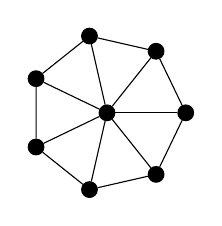
\begin{tikzpicture}
\foreach \i in {0, 1, ..., 6}{
\node[draw, circle, fill = black, inner sep = 2pt] (\i) at (360/7*\i:1){};}
\node[draw, circle, fill = black, inner sep = 2pt] (7) at (0,0){};
\foreach \i in {0, 1, ..., 6}{
\draw let \n1 = {int(mod(\i+1,7))} in (\i) -- (\n1);
\draw (\i) -- (7);}
\end{tikzpicture}
}

\ffigbox{\caption{}\label{}}{
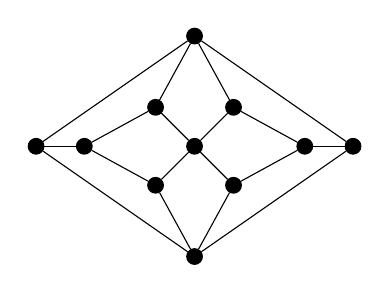
\begin{tikzpicture}[every node/.style={draw, circle, fill = black, 
inner sep = 2pt}]
\foreach \i in {0, 1, 2, 3}{
\node[] (\i) at (360/4*\i+45:.7){};}
\foreach \i in {4, 5, 6, 7}{
\node[] (\i) at (360/4*\i:1.4){};}
\node (8) at (0,0) {};
\node[ right = .4cm of 4]  (9) {};
\node [left = .4cm of 6] (10) {};
\foreach \i/\j in {8/0, 8/1, 8/2, 8/3, 0/5, 5/1, 1/6, 6/2, 2/7, 7/3, 3/4, 5/10, 10/7, 5/9, 9/7, 0/4, 6/10, 4/9}{
\draw (\i) -- (\j);}
\end{tikzpicture}
}

\ffigbox{\caption{}\label{}}{
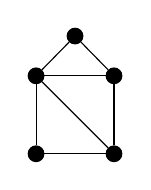
\begin{tikzpicture}[every node/.style={draw, circle, fill = black, 
inner sep = 2pt}]
\foreach \i in {0, 1, 2, 3}{
\node[] (\i) at (360/4*\i+45:.7){};}
\node[draw, circle, fill = black, inner sep = 2pt] (5) at (0,1){};
\foreach \i in {0, 1, ..., 3}{
\draw let \n1 = {int(mod(\i+1,4))} in (\i) -- (\n1);}
\draw (1) -- (5) (5) --(0) (1) -- (3);
\end{tikzpicture}
}

\end{subfloatrow}
\begin{subfloatrow}
\ffigbox{\caption{}\label{}}{
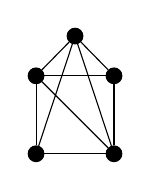
\begin{tikzpicture}[every node/.style={draw, circle, fill = black, 
inner sep = 2pt}]
\foreach \i in {0, 1, 2, 3}{
\node[] (\i) at (360/4*\i+45:.7){};}
\node[draw, circle, fill = black, inner sep = 2pt] (5) at (0,1){};
\foreach \i in {0, 1, ..., 3}{
\draw let \n1 = {int(mod(\i+1,4))} in (\i) -- (\n1);}
\draw (1) -- (5) (5) --(0) (5) -- (2) (5) -- (3) (1)--(3);
\end{tikzpicture}
}

\ffigbox{\caption{}\label{}}{
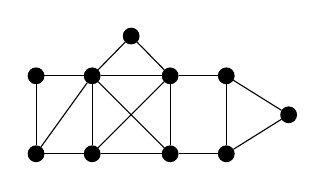
\begin{tikzpicture}[every node/.style={draw, circle, node distance = .5cm, fill = black, 
inner sep = 2pt}]
\foreach \i in {0, 1, 2, 3}{
\node[] (\i) at (360/4*\i+45:.7){};}
\node[] (5) at (0,1){};
\foreach \i in {0, 1, ..., 3}{
\draw let \n1 = {int(mod(\i+1,4))} in (\i) -- (\n1);}
\draw (1) -- (5) (5) --(0) ;
\node[left = of 2] (6){};
\node[left = of 1] (7){};
\node[right = of 0] (8){};
\node[right = of 3] (9){};
\node[] (10) at (2,0) {};
\foreach \i/\j in {1/7, 7/6, 6/2, 1/6, 0/8, 8/9, 9/3, 8/9, 9/10, 1/3, 0/2, 10/8}{
\draw (\i) -- (\j);}
\end{tikzpicture}
}

\end{subfloatrow}
}{
\caption{Determine the chromatic number of the following graphs.}
\label{chromatic}}
\end{center}
\end{figure}


\begin{figure}[htbp]
\begin{center}
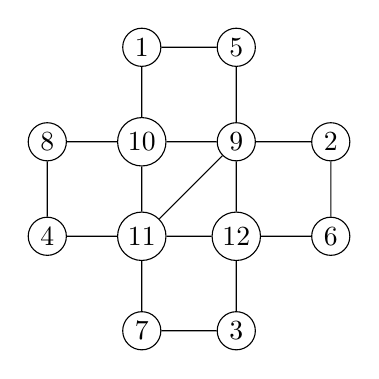
\begin{tikzpicture}[every node/.style={draw, circle, inner sep = 2 pt}, scale=1.2]
\node (1) at (0,2) {1};
\node  (2) at (2,1) {2};
\node  (3) at (1,-1) {3};
\node (4) at (-1,0) {4};
\node (5) at (1,2) {5};
\node (6) at (2,0) {6};
\node (7) at (0,-1) {7};
\node (8) at (-1,1) {8};
\node (9) at (1,1) {9};
\node (10) at (0,1) {10};
\node (11) at (0,0) {11};
\node (12) at (1,0) {12};
\draw (10) -- (1) -- (5) -- (9) -- (2) -- (6) -- (12) -- (3) -- (7) -- (11) -- (4) -- (8) -- (10) -- (9) -- (12) -- (11) -- (10) (11) --(9);
\end{tikzpicture}
\caption{A graph}
\label{greedy}
\end{center}
\end{figure}


\newcommand{\grotzsch}[1]{

\begin{tikzpicture}[every node/.style={draw, circle, fill = black, 
inner sep = 2pt}]
%
\pgfmathtruncatemacro{\result}{#1-1}
\pgfmathtruncatemacro{\endNum}{#1*2}
\pgfmathtruncatemacro{\resultNum}{#1*2-1}
\pgfmathsetmacro{\angle}{360/#1}
%
\foreach \i in {0, 1, ..., \result}{
\node[] (\i) at (\angle*\i:2){};
\path let \n1={int(\i+#1)} in node[]  (\n1) at  (\angle*\i:1){};
}
\node (\endNum) at (0,0){};
\foreach \i in {0, ..., \result}{
\draw let \n1 = {int(mod(\i+1,#1))} in (\i) -- (\n1);
}
\foreach \i in {#1, ..., \resultNum}{
\draw let \n1 = {int(mod(\i+1,#1))} in (\i) -- (\n1);
\draw let \n1 = {int(mod(\i-1,#1))} in (\i) -- (\n1);
\draw (\i) -- (\endNum);
}
\end{tikzpicture}
}

\begin{figure}[htbp]
\begin{center}
\ffigbox{
\begin{subfloatrow}[2]
\ffigbox{\caption{The Gr\"otzsch graph $G_{5}$}\label{grotzsch}}{
%\begin{tikzpicture}[every node/.style={draw, circle, fill = black, 
%inner sep = 2pt}]
%\foreach \i in {0, 1, ..., 4}{
%\node[] (\i) at (360/5*\i:2){};
%\path let \n1={int(\i+5)} in node[]  (\n1) at  (360/5*\i:1){};}
%\node (10) at (0,0){};
%\foreach \i in {0, ..., 4}{
%\draw let \n1 = {int(mod(\i+1,5))} in (\i) -- (\n1);
%}
%\foreach \i in {5, ..., 9}{
%\draw let \n1 = {int(mod(\i+1,5))} in (\i) -- (\n1);
%\draw let \n1 = {int(mod(\i-1,5))} in (\i) -- (\n1);
%\draw (\i) -- (10);
%}
%\end{tikzpicture}
\grotzsch{5}
}


\ffigbox{\caption{Graph $G_{6}$}\label{grotzsch6}}{
\grotzsch{6}
}

%\ffigbox{\caption{Graph $G_{7}$}\label{grotzsch7}}{\grotzsch{7}
%}

\end{subfloatrow}
}{
\caption{The Gr\"otzsch graph and a generalization}
\label{}}
\end{center}
\end{figure}




\end{document}